\documentclass[fleqn]{beamer}
\beamertemplatenavigationsymbolsempty

\usepackage[T1]{fontenc}
\usepackage[utf8]{inputenc}

\usepackage{amsmath,amssymb}
\usepackage{graphicx}
\usepackage{mathptmx}
\usepackage{subcaption}
\usepackage{amsthm}
\usepackage{tikz}
%\usepackage[colorlinks=true,naturalnames=true,plainpages=false,pdfpagelabels=true]{hyperref}
\usetikzlibrary{patterns,decorations.pathmorphing,positioning, arrows, chains}

\usepackage[backend=biber, sorting=none]{biblatex}
\addbibresource{uni.bib}

\setbeamertemplate{endpage}{%
    \begin{frame}
        \centering
        \Large \emph{To be continued\ldots}

        \vspace{1cm}

        \centering
        \Large \emph{Thank You!}
    \end{frame}
}

\AtEndDocument{\usebeamertemplate{endpage}}

% vertical separator macro
\newcommand{\vsep}{
  \column{0.0\textwidth}
    \begin{tikzpicture}
      \draw[very thick,black!10] (0,0) -- (0,7.3);
    \end{tikzpicture}
}
\setlength{\mathindent}{0pt}

% Beamer theme
\usetheme{UniVienna}
\usefonttheme[onlysmall]{structurebold}
\mode<presentation>
\setbeamercovered{transparent=10}

\title
{SGD with Large Step Sizes Learns Sparse Features}
\subtitle{Seminar Optimization}
\author[Popović Milutin]
{Popović Milutin\newline\newline Supervisor: Radu Ioan Bot}
\date{31. October 2023}

\begin{document}
    \begin{frame}
        \titlepage
    \end{frame}

    \begin{frame}{SGD (Stochastic gradient descent)}
        \begin{itemize}
            \item Objective is to minimize functions of the
                form
                \begin{align*}
                    \hspace{0.3\linewidth}
                    f(x) = \frac{1}{n} \sum_{i=1}^{n} f_i(x)
            \end{align*}
        \end{itemize}
    \end{frame}

    \begin{frame}{SGD (Stochastic gradient descent)}
        \begin{itemize}
            \item Training Data:
                \begin{align*}
                    \hspace{0.3\linewidth}
                    \{(x_1, y_1),\ldots,(x_n,y_n)\} \in \mathbb{R}^{d} \times
                    \mathcal{Y}
            \end{align*}
        \item \mbox{}\onslide<2->{In large-scale ML: large dimension $d$\newline
            and large number of training data $n$.}
        \end{itemize}
    \end{frame}

    \begin{frame}{SGD (Stochastic gradient descent)}
        Classical examples of fitting the data via minimizing:
        \begin{itemize}
            \item \mbox{}\onslide<2->{Least Squares
                \begin{align*}
                    \hspace{0.3\linewidth}
                    \frac{1}{n} \| Ax - b \|_2^2 =\frac{1}{n}\sum_{i=1}^n(a_i^T x - b_i)^2
            \end{align*}}
            \item \mbox{}\onslide<3->{Support Vector Machine (SVM):
                \begin{align*}
                    \hspace{0.3\linewidth}
                    \frac{1}{2}||x||_2^2 + \frac{C}{n} \sum_i^n max(0, 1 - y_i(x^T a_i + b))
            \end{align*}}
        \item \mbox{}\onslide<4->{Deep Neural Nets
                \begin{align*}
                    \hspace{0.3\linewidth}
                    \frac{1}{n} \sum_i^n \text{loss}(y_i, DNN(x; a_i))
                \end{align*}}

        \end{itemize}
    \end{frame}

    \begin{frame}{SGD (Stochastic gradient descent)}
        \begin{itemize}
            \item Common pattern:
                \begin{align*}
                    \hspace{0.3\linewidth}
                    f(x) = \frac{1}{n} \sum_{i=1}^{n} f_i(x)
                \end{align*}
        \end{itemize}
    \end{frame}

    \begin{frame}{GD vs SGD}
        \begin{itemize}
            \item \mbox{}\onslide<2->{GD would compute the gradient of every $f_i(x)$ to update the
                next iterate}
            \item \mbox{}\onslide<3->{SGD picks a pseudorandom $i(r) \in \{1,
                2, \ldots, n\}$}
            \item \mbox{}\onslide<4->{then uses only $\nabla f_{i(r)}(x_k)$ as its descent
                direction
                \begin{align*}
                    \hspace{0.3\linewidth}
                    x^{k+1} = x^{k} - t_k \nabla f_{i(r)}(x^{k})
            \end{align*}}

        \item \mbox{}\onslide<5->{
            Key property : $\mathbb{E}[\nabla f_{i(r)}(x)] = \nabla f(x)$}
        \item  \mbox{}\onslide<5->{
            $\nabla f_{i(r)}(x)$ is an unbiased estimator !
            }
        \end{itemize}
    \end{frame}

    \begin{frame}{Large stepsizes induce Sparse Features}
        \begin{itemize}
            \item  \mbox{}\onslide<1->{large step sizes -> \textit{loss
                stabilization}}
            \item \mbox{}\onslide<2->{the longer the larger step size is used
                the better the sparse representation}
        \end{itemize}

        \begin{figure}[H]
            \centering
            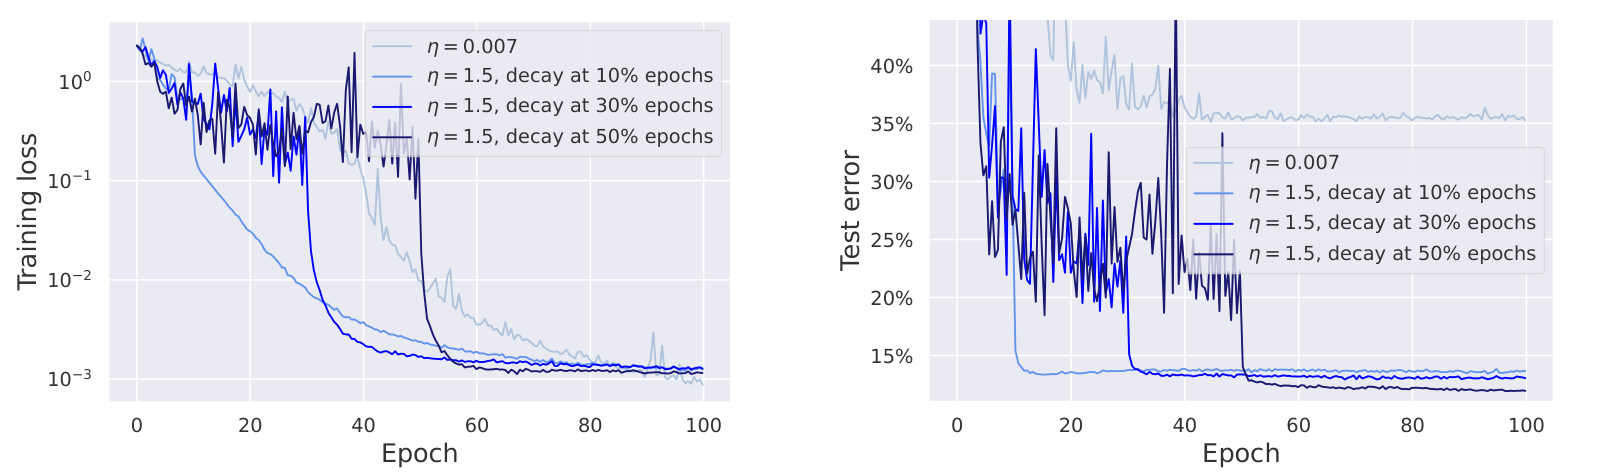
\includegraphics[width=0.9\textwidth]{./pics/resnet18.png}
            \caption{ResNet-18 (Residual Network with 18 layers) trained on
            CIFAR-10 (60k 32x32 images)} \cite{andriushchenko2023sgd}
        \end{figure}
    \end{frame}

    \begin{frame}{Bibliography}
        \nocite{andriushchenko2023sgd}
        \printbibliography
    \end{frame}
\end{document}
